% Template for Carleton problem sets
% Author: Andrew Gainer-Dewar, 2013
% This work is licensed under the Creative Commons Attribution 4.0 International License.
% To view a copy of this license, visit http://creativecommons.org/licenses/by/4.0/ or send a letter to Creative Commons, 444 Castro Street, Suite 900, Mountain View, California, 94041, USA.

% Kevin Gilbert and Gilberto Rodriguez
% Lab 2 7-Feb-2014 EE445L
\documentclass[11pt]{article}
\usepackage{ccpset}
\usepackage{graphicx, lmodern, textcomp}
\usepackage{amsmath}

% The Latin Modern font is a modernized replacement for the classic
% Computer Modern. Feel free to replace this with a different font package.
\usepackage{lmodern}

\title{EE445L - Lab 02 Report}
\author{Kevin Gilbert\\ Gilberto Rodriguez}
\date{\today}
\prof{Professor Bard}
\course{Lab: Monday/Wednesday 5-6:15}

\begin{document}
\maketitle{}

\section*{Ojective}
•To develop software debugging techniques\\
\indent- Performance debugging (dynamic or real time)\\
\indent- Profiling (detection and visualization of program activity)\\
• To pass data using a FIFO queue,\\
• To learn how to use the oscilloscope and logic analyzer,\\
• To observe critical sections,\\
• Get an early start on Lab 3, by writing a line drawing function.\\

\section*{Mesurement Data}


\underline{0x000009C4 4601 MOV r1,r0}\\
\underline{0x000009C6 481D LDR r0,[pc,\#116] ; @0x0A3C}\\
\underline{0x000009C8 6800 LDR r0,[r0,\#0x00]}\\
\underline{0x000009CA 4A1B LDR r2,[pc,\#108] ; @0x0A38}\\
\underline{0x000009CC 6812 LDR r2,[r2,\#0x00]}\\
\underline{0x000009CE 4290 CMP r0,r2}\\
\underline{0x000009D0 D101 BNE 0x000009D6}\\
0x000009D2 2000 MOVS r0,\#0x00\\
\underline{0x000009D4 4770 BX lr}\\
\underline{0x000009D6 4818 LDR r0,[pc,\#96] ; @0x0A38}\\
\underline{0x000009D8 6800 LDR r0,[r0,\#0x00]}\\
\underline{0x000009DA 7800 LDRB r0,[r0,\#0x00]}\\
\underline{0x000009DC 7008 STRB r0,[r1,\#0x00]}\\
\underline{0x000009DE 4816 LDR r0,[pc,\#88] ; @0x0A38}\\
\underline{0x000009E0 6800 LDR r0,[r0,\#0x00]}\\
\underline{0x000009E2 1C40 ADDS r0,r0,\#1}\\
\underline{0x000009E4 4A14 LDR r2,[pc,\#80] ; @0x0A38}\\
\underline{0x000009E6 6010 STR r0,[r2,\#0x00]}\\
\underline{0x000009E8 4610 MOV r0,r2}\\
\underline{0x000009EA 6802 LDR r2,[r0,\#0x00]}\\
\underline{0x000009EC 4811 LDR r0,[pc,\#68] ; @0x0A34}\\
\underline{0x000009EE 3020 ADDS r0,r0,\#0x20}\\
\underline{0x000009F0 4282 CMP r2,r0}\\
\underline{0x000009F2 D102 BNE 0x000009FA}\\
0x000009F4 3820 SUBS r0,r0,\#0x20\\
0x000009F6 4A10 LDR r2,[pc,\#64] ; @0x0A38\\
0x000009F8 6010 STR r0,[r2,\#0x00]\\
\underline{0x000009FA 2001 MOVS r0,\#0x01}\\
\underline{0x000009FC E7EA B 0x000009D4}\\[.25in]
0x00000A34 00FC LSLS r4,r7,\#3\\
0x00000A36 2000 MOVS r0,\#0x00\\
0x00000A38 0034 MOVS r4,r6\\
0x00000A3A 2000 MOVS r0,\#0x00\\
0x00000A3C 0030 MOVS r0,r6\\
0x00000A3E 2000 MOVS r0,\#0x00

\begin{equation*}
36 cycles \times (1 \div 50 MHz) = .72 \mu s\\
\end{equation*}
\vskip 0.5in

  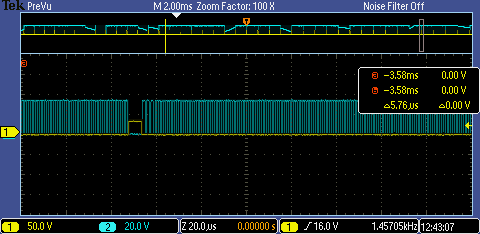
\includegraphics[width=1\textwidth]{TEK00001}\\[.25in]
  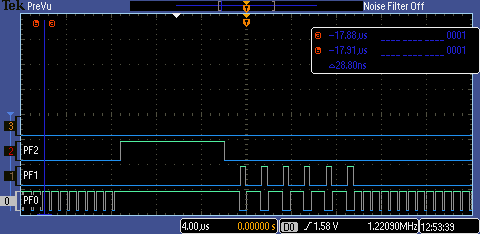
\includegraphics[width=1\textwidth]{TEK00003}\\[.25in]
  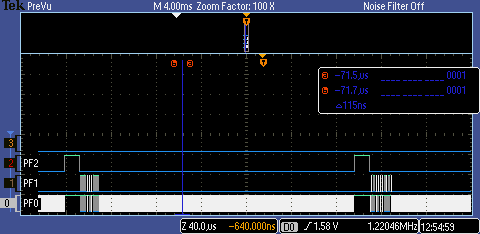
\includegraphics[width=1\textwidth]{TEK00004}\\[.25in]
  Part B and C: When the interrupt is triggered, the code in the foreground in put on pause. The interrput handler then takes care of it's assigned code. This way, RxFifo\_Put is never executed with RxFifo\_Get.\\
  
  \centerline{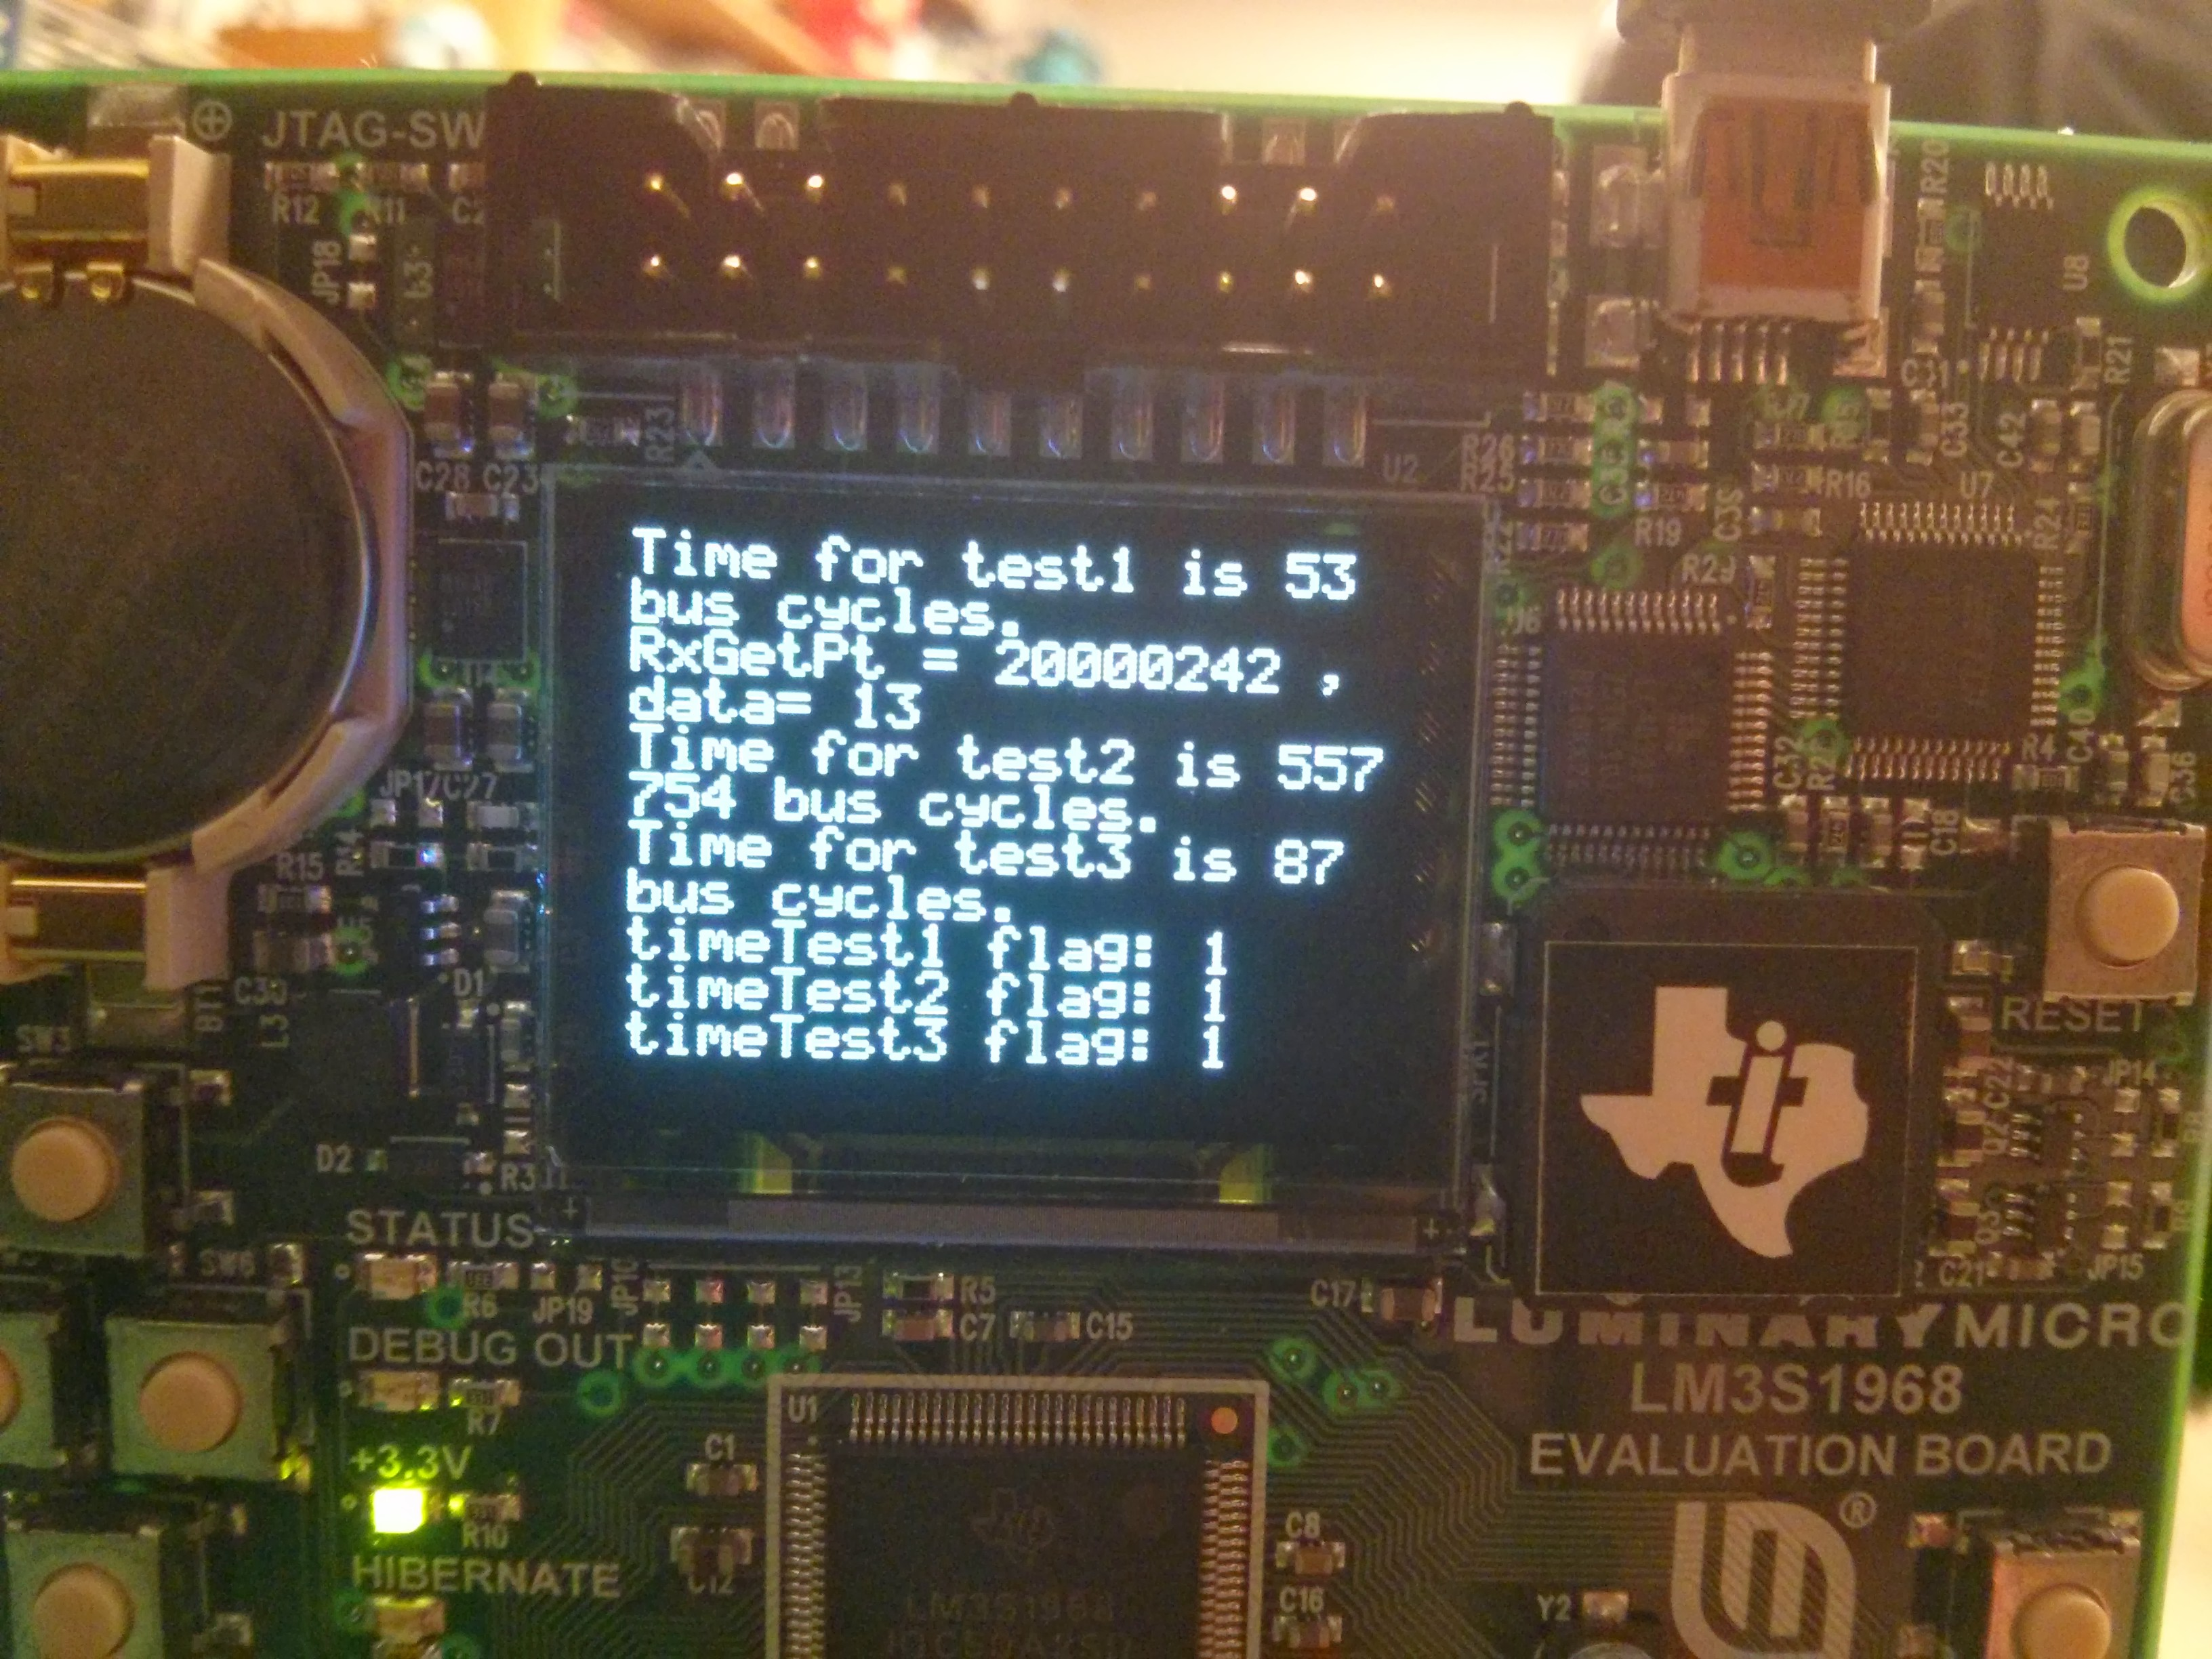
\includegraphics[width=1\textwidth]{lab2_partDoled}\\[.25in]}
  Part D\\

 \centerline{ 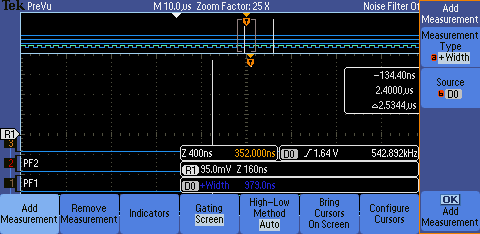
\includegraphics[width=1\textwidth]{TEK00005}\\[.25in]}
  \centerline{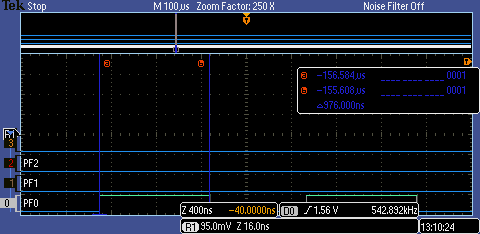
\includegraphics[width=1\textwidth]{TEK00007}\\[.25in]}
 \centerline{ 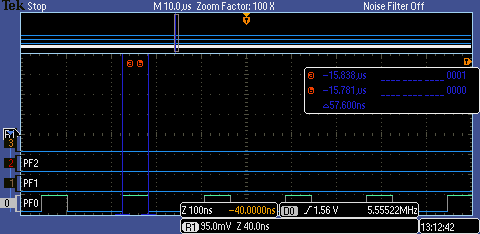
\includegraphics[width=1\textwidth]{TEK00008}\\[.25in]} 
  Part E: Refer to Problem 1
  \begin{equation*}
  976ns - 57.6ns = 918.4 ns
  \end{equation*}
  \centerline{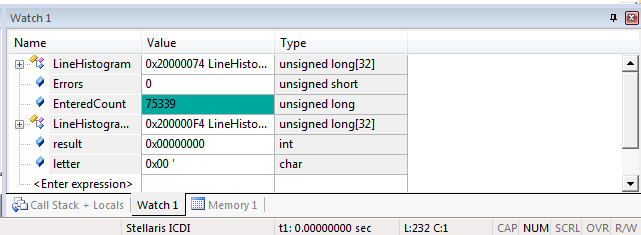
\includegraphics[width=1\textwidth]{critSectionsRxFIFO}\\[.25in]}
  Part F\\

  \centerline{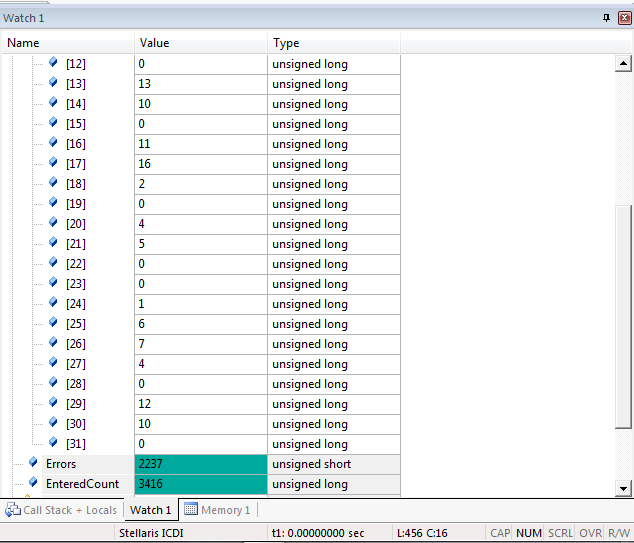
\includegraphics[width=1\textwidth]{badCritSec}\\[.25in]}
  Part G\\

  \centerline{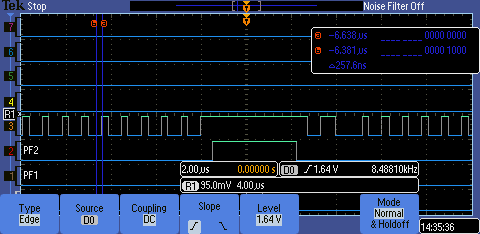
\includegraphics[width=1\textwidth]{TEK00009}\\[.25in]}
  \centerline{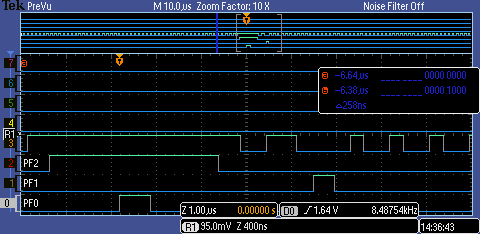
\includegraphics[width=1\textwidth]{TEK00013}\\[.25in]}
  Part H:\\
  \begin{gather*}
  PF0 \to TxFifo\_ Put\\
	PF1 \to Main\: Loop (checks\: for\: errors)\\
	PF2 \to Timer\: Interrupt\\
	PF3 \to TxFifo\_Get
\end{gather*}

\vskip 0.25in

\section*{Analysis and Discussion}
\begin{pset}
  \problem{1}
  You measured the execution speed of RxFifo\textunderscore Get three ways. Did you get 
the same result? If not, explain.\\
\textit{We did not get the same results. Timing method one of reading the dissambly and counting instructions was the most time consuming and least efficienent; due to piping and profiling techniques on the board, execution times may differ. The next two timing techniques involved measuring with the systick timer, and by setting GPIO pins high/low and measuring with an oscilliscope. The first method with systick counted 53 cycles of execution at 20ns, providing us with a 1020ns execution time. The second method of using the GPIO pins provided a pulse width of 976ns. We then measured the time it took to set a pin high and low, which came out to 57.6ns. Therefore the GPIO method provided us with a run time of 918.4ns. The overhead of measuring the systick register added the slight drift in measurement times. The difference was about 100ns, or 5 bus cycles. This would match up with the overhead of reading a register and masking the data.}

  \problem{2}
  Which method of measuring execution speed would you use if you expected the execution speed to vary a lot (e.g., ranging from 0.5 to 20ms), and wanted to determine the minimum, maximum and average speed? Why?\\
\textit{Measuring varying pulsewidths on a logic analyser can be difficult. It also requires being around a logic analyser. It would be much simpler to dump execution times into an array using systick measurements, and then run averages on that data.}

  \problem{3}Which method of measuring execution speed would you use if you expected the execution speed to be very large (e.g., 20 seconds)? Why?\\
\textit{For very large values, you should use an oscilloscope since systick will overflow and reset.}

  \problem{4}Define “minimally intrusive”.\\
\textit{Debugging techniques that have minumum overhead. In other words, the software should run nearly the same as if the debugging tools were not present, in real time. Printf and using breakpoints are examples of intrusive debugging.}

  \problem{5}List the two necessary components collected during a “profile”.\\
\textit{Profilers collects time history of program execution. Two necessary components are the location and time that a thread executes. Data involved in the execution may also be logged.}

  \problem{6}What is the critical section in the bad FIFO? How would you remove the critical section?\\
\textit{BadFifo does not use a volatile put pointer for one, the data pointer may be corrupted if interrupted during its execution. A start and end critical section can also be placed around sections handling data.}

\end{pset}



\end{document}